% Presentación final · TPE Redes de Información · Grupo 6
%
%   make            -> presentacion.pdf
%
% Qué contar en cada diapositiva, quién habla y cuánto tiempo va en \note{} (no se imprime).
% Lo marcado con TODO falta completar o decidir.

\documentclass[aspectratio=169,11pt]{beamer}

\usepackage[spanish,es-noshorthands]{babel}
\usepackage[utf8]{inputenc}
\usepackage[T1]{fontenc}
\usepackage{amssymb}
\usepackage{booktabs}
\usepackage{tikz}
\usetikzlibrary{arrows.meta,positioning,fit}

\usetheme[progressbar=frametitle,numbering=fraction]{metropolis}

% Oradores: reemplazar por los nombres cuando se decida el reparto.
\newcommand{\oradorA}{Orador A}
\newcommand{\oradorB}{Orador B}
\newcommand{\oradorC}{Orador C}

% Encabezado del guion: \guion{orador}{tiempo}
\newcommand{\guion}[2]{\textbf{#1 · #2}\par\medskip}

\newcommand{\cmd}[1]{\texttt{\small #1}}

\title{The Store sobre K3s gestionado con Ansible}
\subtitle{Tema 5 · Despliegue y gestión del clúster de Kubernetes}
\author{Grupo 6 · Nicolás Arancibia Carabajal · Lautaro Paletta · Agustín Ronda}
\institute{Redes de Información · ITBA · 2C 2026}
\date{}

\begin{document}

% ---------------------------------------------------------------------------
% Apertura
% ---------------------------------------------------------------------------

\begin{frame}
  \titlepage
\end{frame}
\note{
  \guion{\oradorA}{0:20}
  \begin{itemize}
    \item Presentar al grupo y el tema en una frase: ``automatizamos el ciclo de vida del clúster
      donde corre The Store''.
    \item Avisar que la mitad de la presentación es demo en vivo.
  \end{itemize}
}

\begin{frame}{Agenda}
  \begin{enumerate}
    \item Problemática: cómo se opera hoy The Store
    \item Solución: diseño, arquitectura de red y tecnologías
    \item Demo: los cinco casos de uso de la pre-entrega
    \item Resultados, limitaciones y conclusiones
  \end{enumerate}
\end{frame}
\note{
  \guion{\oradorA}{0:25}
  \begin{itemize}
    \item Recorrer rápido. Mencionar quién presenta cada bloque.
  \end{itemize}
}

% ---------------------------------------------------------------------------
% Problemática
% ---------------------------------------------------------------------------

\section{Problemática}

\begin{frame}{The Store hoy}
  \begin{columns}[T]
    \column{0.5\textwidth}
      Tienda online con cinco microservicios:
      \begin{itemize}
        \item \textbf{ui} · Java (Spring Boot)
        \item \textbf{catalog} · Go
        \item \textbf{cart} · Java (Spring Boot)
        \item \textbf{orders} · Java (Spring Boot)
        \item \textbf{checkout} · Node.js (NestJS)
      \end{itemize}
    \column{0.5\textwidth}
      Se despliega con \cmd{local.sh}:
      \begin{enumerate}
        \item crea un clúster de \textbf{Kind} en una sola máquina,
        \item carga las imágenes con \cmd{kind load},
        \item aplica los manifiestos.
      \end{enumerate}
      \medskip
      \alert{Pensado para desarrollar, no para operar.}
  \end{columns}
\end{frame}
\note{
  \guion{\oradorA}{1:00}
  \begin{itemize}
    \item Qué es The Store en dos frases. No detenerse en los microservicios: el tema no es la
      aplicación sino la plataforma donde corre.
    \item Cómo se despliega hoy: un script, un clúster Kind, un solo nodo.
    \item Remarcar \cmd{kind load}: solo existe en Kind, y más adelante explica por qué usamos un registry.
  \end{itemize}
}

\begin{frame}{Problemática y objetivo}
  \begin{itemize}
    \item Cada operación sobre el clúster se hace \textbf{a mano} y depende de quién la ejecute.
    \item No se pueden \textbf{agregar ni quitar nodos}: hay que borrar el clúster y recrearlo,
      con la tienda fuera de servicio.
    \item Ante un pico de tráfico (Black Friday, Navidad) no hay forma rápida de \textbf{sumar capacidad}.
  \end{itemize}
  \begin{alertblock}{Objetivo}
    Un clúster que cualquier integrante del equipo pueda \textbf{crear}, \textbf{ampliar},
    \textbf{reducir} y \textbf{reconstruir} desde cero, de forma automatizada y repetible.
  \end{alertblock}
\end{frame}
\note{
  \guion{\oradorA}{1:30}
  \begin{itemize}
    \item Frase clave: ``el problema está en la plataforma, no en la aplicación''.
    \item Los cuatro verbos del objetivo (crear, ampliar, reducir, reconstruir) son los casos de
      uso de la demo: anticiparlo para que el público los reconozca después.
    \item Pase a \oradorB: ``veamos cómo lo diseñamos''.
  \end{itemize}
}

% ---------------------------------------------------------------------------
% Solución
% ---------------------------------------------------------------------------

\section{Solución}

\begin{frame}{Diseño en tres capas}
  \centering
  \begin{tikzpicture}[
      capa/.style={draw, rounded corners, minimum width=8cm, minimum height=1.1cm, align=center},
      every node/.style={font=\small}]
    \node[capa, fill=green!10] (app) {\textbf{Aplicación} · The Store, imágenes en GitHub Container Registry};
    \node[capa, fill=blue!10, below=0.25cm of app] (k8s) {\textbf{Clúster} · K3s: 1 server (control plane) + N agents (workers)};
    \node[capa, fill=gray!15, below=0.25cm of k8s] (nodos) {\textbf{Nodos} · contenedores Docker \texttt{rancher/k3s} en la red \texttt{k3s-net}};
    \node[draw, rounded corners, fill=orange!20, minimum width=2.6cm, align=center,
          left=0.6cm of k8s, minimum height=3.8cm] (ansible)
          {\textbf{Ansible}\\[2pt] inventario\\+\\playbooks};
    \draw[-{Latex}, thick] (ansible.east |- app) -- (app.west);
    \draw[-{Latex}, thick] (ansible.east |- k8s) -- (k8s.west);
    \draw[-{Latex}, thick] (ansible.east |- nodos) -- (nodos.west);
  \end{tikzpicture}

  \medskip
  Ansible crea los nodos, instala el clúster y despliega la aplicación.\\
  Desde ahí, Kubernetes mantiene la tienda corriendo y reparte los pods entre los nodos.
\end{frame}
\note{
  \guion{\oradorB}{1:00}
  \begin{itemize}
    \item Leer de abajo hacia arriba: nodos, clúster, aplicación.
    \item Ansible actúa sobre las tres capas; el inventario dice qué nodos existen, con nombre, rol e IP.
    \item Hay un playbook por operación: crear, desplegar, agregar, quitar y destruir.
  \end{itemize}
}

\begin{frame}{Arquitectura de red}
  \centering
  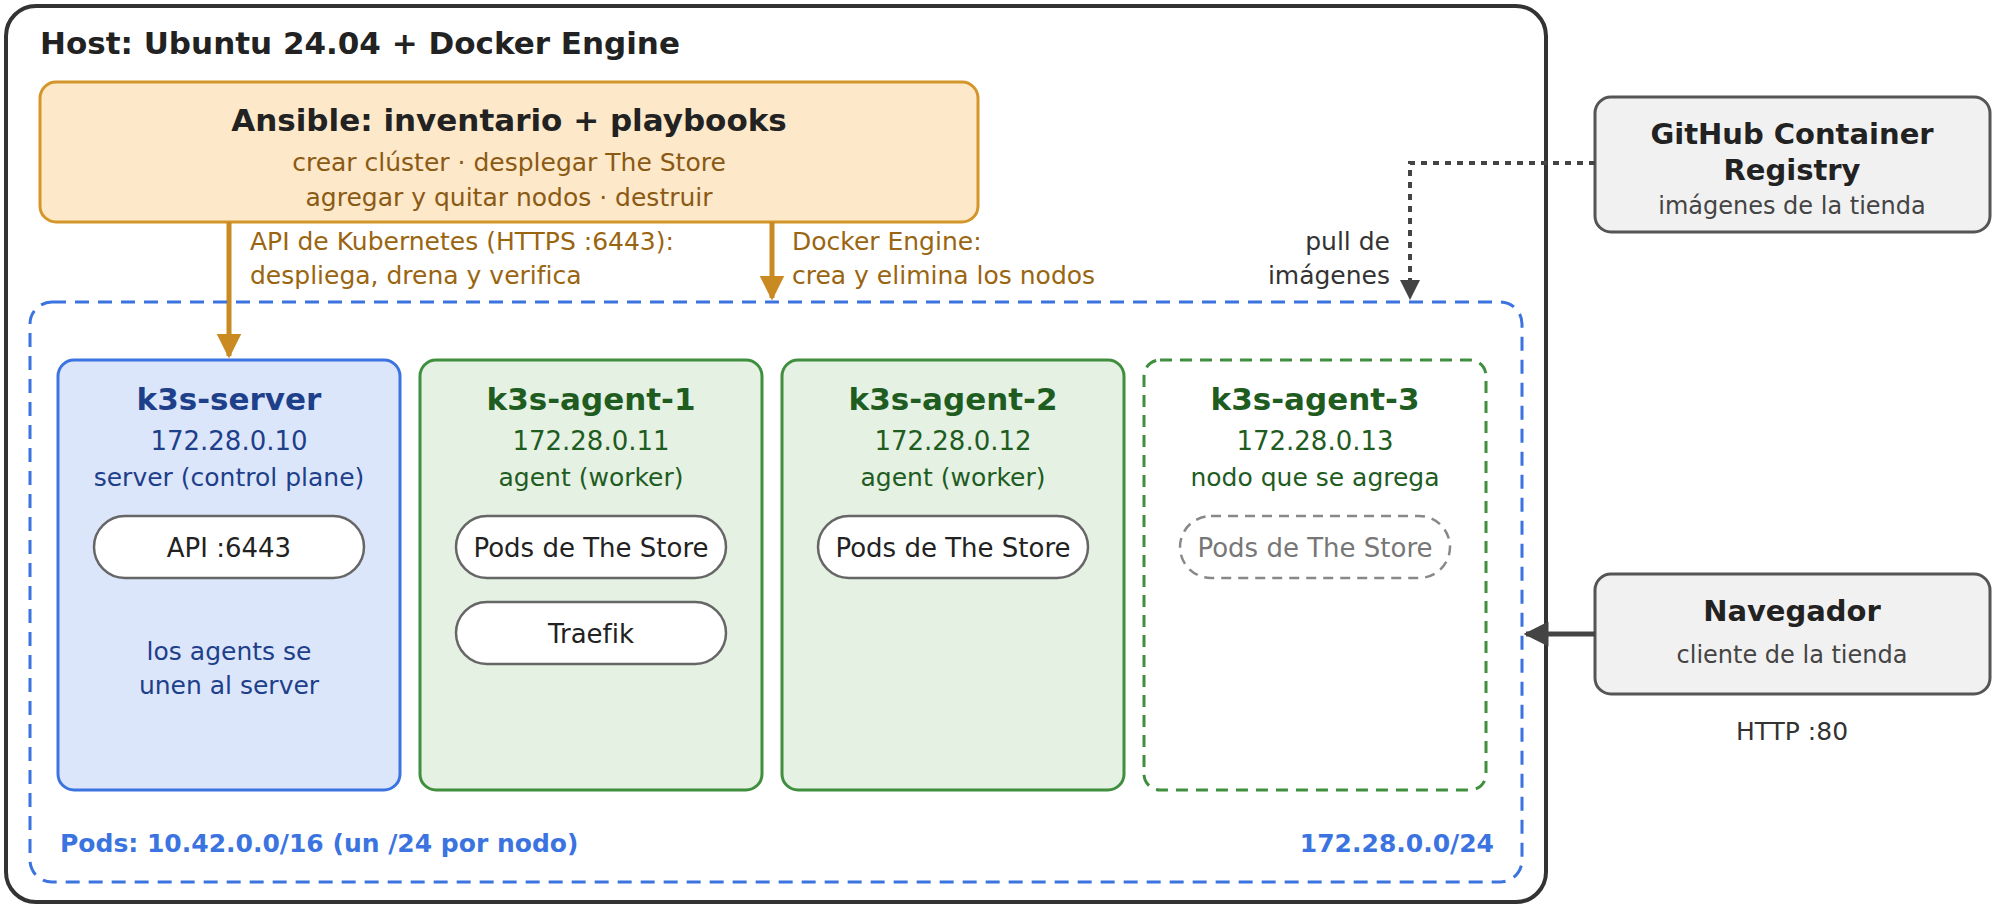
\includegraphics[width=0.86\textwidth]{../diagrama/arquitectura-k3s.png}

  \small
  \texttt{k3s-net} 172.28.0.0/24 (gw .1) · Pods 10.42.0.0/16 (un /24 por nodo) ·
  Services 10.43.0.0/16
\end{frame}
\note{
  \guion{\oradorB}{2:00}
  \begin{itemize}
    \item Recorrer de afuera hacia adentro: host Ubuntu 24.04 con Docker Engine; Ansible corre en
      el host.
    \item Red Docker propia \texttt{k3s-net} 172.28.0.0/24; cada nodo con IP fija del inventario
      (.10 server, .11 y .12 workers).
    \item \texttt{k3s-agent-3} punteado: es el nodo que se suma en el caso 3.
    \item Dos redes internas de Kubernetes: pods 10.42.0.0/16 (un /24 por nodo) y Services
      10.43.0.0/16 (no figura en el diagrama, decirlo).
    \item Afuera: GHCR, de donde cada nodo descarga las imágenes, y el navegador, que entra por
      HTTP :80.
  \end{itemize}
}

\begin{frame}{Flujos de red}
  \centering
  \footnotesize
  \begin{tabular}{@{}lll@{}}
    \toprule
    \textbf{Origen $\rightarrow$ destino} & \textbf{Protocolo} & \textbf{Para qué} \\
    \midrule
    Ansible $\rightarrow$ Docker Engine & API Docker (socket Unix) & crea y elimina los nodos \\
    Ansible $\rightarrow$ \texttt{k3s-server} & HTTPS · TCP 6443 & despliega, drena y verifica \\
    agents $\rightarrow$ \texttt{k3s-server} & HTTPS · TCP 6443 + token & unión al clúster \\
    pod $\leftrightarrow$ pod (entre nodos) & VXLAN · UDP 8472 (Flannel) & red de pods 10.42.0.0/16 \\
    nodos $\rightarrow$ \texttt{ghcr.io} & HTTPS · TCP 443 (NAT del host) & descarga de imágenes \\
    navegador $\rightarrow$ cualquier nodo & HTTP · TCP 80 & ServiceLB $\rightarrow$ Traefik $\rightarrow$ ui \\
    \bottomrule
  \end{tabular}
\end{frame}
\note{
  \guion{\oradorB}{1:00}
  \begin{itemize}
    \item Esta tabla es el resumen ``de Redes'': quién habla con quién, por qué protocolo y puerto.
    \item Remarcar que Ansible usa dos APIs distintas: la de Docker para la capa de nodos y la de
      Kubernetes para la de clúster y aplicación.
    \item Los agents se autentican con el token compartido que Ansible genera una sola vez.
  \end{itemize}
}

\begin{frame}{Recorrido de un request}
  \centering
  \begin{tikzpicture}[
      paso/.style={draw, rounded corners, fill=blue!8, align=center, font=\footnotesize,
                   minimum height=1.1cm, text width=2.35cm},
      flecha/.style={-{Latex}, thick}]
    \node[paso, fill=gray!15] (nav) {Navegador\\(en el host)};
    \node[paso, right=0.45cm of nav] (svclb) {\texttt{172.28.0.12:80}\\ServiceLB (hostPort)};
    \node[paso, right=0.45cm of svclb] (traefik) {Service \texttt{traefik}\\10.43.x.x};
    \node[paso, right=0.45cm of traefik] (tpod) {Pod Traefik\\10.42.1.x};
    \node[paso, below=0.9cm of tpod] (ingress) {Ingress\\\texttt{/} $\rightarrow$ \texttt{ui}};
    \node[paso, left=0.45cm of ingress] (ui) {Pod \texttt{ui}\\10.42.2.x};
    \node[paso, left=0.45cm of ui] (dns) {\texttt{catalog} vía CoreDNS\\10.43.x.x};
    \node[paso, left=0.45cm of dns] (cat) {Pod \texttt{catalog}\\10.42.x.x};
    \draw[flecha] (nav) -- (svclb);
    \draw[flecha] (svclb) -- (traefik);
    \draw[flecha] (traefik) -- (tpod);
    \draw[flecha] (tpod) -- (ingress);
    \draw[flecha] (ingress) -- (ui);
    \draw[flecha] (ui) -- (dns);
    \draw[flecha] (dns) -- (cat);
  \end{tikzpicture}

  \medskip
  \small Si el pod destino está en otro nodo, el paquete viaja encapsulado en VXLAN sobre \texttt{k3s-net}.
\end{frame}
\note{
  \guion{\oradorB}{1:15}
  \begin{itemize}
    \item Seguir un request de punta a punta: entra por el puerto 80 de cualquier nodo, ServiceLB
      lo pasa al Service de Traefik, Traefik aplica el Ingress y lo manda al pod de la UI.
    \item La UI llama a catalog, cart, etc.\ por nombre: CoreDNS resuelve a la IP del Service
      (10.43.x.x) y kube-proxy (iptables) elige un pod.
    \item Si el pod está en otro nodo, Flannel encapsula en VXLAN. Por eso da igual a qué nodo
      entre el request.
    \item TODO: reemplazar las IPs genéricas por las reales con \cmd{kubectl get pods,svc -o wide}.
    \item Pase a \oradorC.
  \end{itemize}
}

\begin{frame}{Decisiones técnicas}
  \small
  \begin{description}[Nodos como contenedores]
    \item[Ansible] compara el estado actual con el deseado y cambia solo la diferencia.
      Re-ejecutar no rompe nada y agregar un nodo no toca a los demás.
    \item[Nodos como contenedores] arrancan en segundos y consumen una fracción de una VM.
      El rol \texttt{docker\_node} está aislado: se puede cambiar por VMs.
    \item[Registry (GHCR)] cada nodo descarga las imágenes por su cuenta; un nodo nuevo no
      depende de que le copien nada (reemplaza a \texttt{kind load}).
    \item[Traefik + ServiceLB] vienen con K3s y publican el puerto 80 en cada nodo, sin instalar
      ni exponer ingress-nginx aparte.
  \end{description}
\end{frame}
\note{
  \guion{\oradorC}{1:15}
  \begin{itemize}
    \item Una frase por decisión, siempre con el ``por qué''.
    \item Ansible vs.\ script: un script ejecuta siempre los mismos pasos; Ansible describe el estado
      deseado. Esto se va a ver en la demo con \texttt{changed=0}.
    \item Contenedores privilegiados: K3s los necesita para administrar la red y los cgroups de los pods.
  \end{itemize}
}

\begin{frame}[fragile]{Ansible: inventario, roles y playbooks}
  \begin{columns}[T]
    \column{0.42\textwidth}
\begin{verbatim}
inventory/hosts.yml
  k3s_server:
    k3s-server  172.28.0.10
  k3s_agents:
    k3s-agent-1 172.28.0.11
    k3s-agent-2 172.28.0.12

roles/
  docker_node/  crea la "máquina"
  k3s/          API, kubeconfig, Ready
  the_store/    manifiestos
\end{verbatim}
    \column{0.55\textwidth}
      \small
      \begin{tabular}{ll}
        \toprule
        \textbf{Playbook} & \textbf{Caso} \\
        \midrule
        \texttt{create-cluster.yml} & 1 · Reproducibilidad \\
        \texttt{deploy-store.yml}   & 2 · Validación \\
        \texttt{add-nodes.yml}      & 3 · Capacidad \\
        \texttt{remove-node.yml}    & 4 · Mantenimiento \\
        \texttt{destroy.yml}        & 5 · Reconstrucción \\
        \bottomrule
      \end{tabular}

      \medskip
      Colecciones: \texttt{community.docker} y \texttt{kubernetes.core}.
  \end{columns}
\end{frame}
\note{
  \guion{\oradorC}{1:15}
  \begin{itemize}
    \item El inventario es la fuente de verdad: qué nodos existen, con su rol (grupo) e IP.
    \item Cada ``host'' del inventario es un nodo-contenedor; Ansible corre en el host con
      conexión local y le habla a la API de Docker y a la de Kubernetes.
    \item Un playbook por caso de uso: la demo sigue exactamente esta tabla.
  \end{itemize}
}

\begin{frame}{Alternativas consideradas}
  \small
  \begin{tabular}{p{0.2\textwidth}p{0.33\textwidth}p{0.37\textwidth}}
    \toprule
    \textbf{Alternativa} & \textbf{Qué ofrece} & \textbf{Por qué no} \\
    \midrule
    kops en AWS & Máquinas, red y clúster; escalado y backup integrados & Costo, un solo proveedor, Ansible pierde su rol \\
    Minikube & Un comando crea todo & SO y red propios: nada que diseñar ni automatizar \\
    Kind / k3d & Nodos en Docker, como el nuestro & Kind no agrega ni quita nodos; k3d lo hace con sus propios comandos \\
    VMs (Multipass o nube) & Lo más parecido a producción & Minutos por VM, $\geq$ 2 GB de RAM por nodo, costo en la nube \\
    \bottomrule
  \end{tabular}
\end{frame}
\note{
  \guion{\oradorC}{1:00}
  \begin{itemize}
    \item Las VMs fueron nuestra primera opción: contar por qué cambiamos (tiempos y RAM en una notebook).
    \item Todas las alternativas descartadas le quitaban trabajo a Ansible, que es el corazón del tema.
    \item Pase a \oradorA\ para la demo.
  \end{itemize}
}

% ---------------------------------------------------------------------------
% Demo
% ---------------------------------------------------------------------------

\section{Demo}

\begin{frame}{Scope del POC: cinco casos de uso}
  \small
  \begin{tabular}{clp{0.55\textwidth}}
    \toprule
    \textbf{\#} & \textbf{Caso} & \textbf{Criterio de éxito} \\
    \midrule
    1 & Reproducibilidad & 3 nodos Ready; la 2ª ejecución no cambia nada \\
    2 & Validación & Pods Running repartidos entre nodos; la tienda abre \\
    3 & Capacidad & Solo cambia el nodo nuevo; 4 nodos Ready \\
    4 & Mantenimiento & El nodo se va; sus pods corren en otros; la tienda sigue abriendo \\
    5 & Reconstrucción & Destroy no deja nada; el rebuild llega al estado de 1 y 2 \\
    \bottomrule
  \end{tabular}
\end{frame}
\note{
  \guion{\oradorA}{0:30}
  \begin{itemize}
    \item ``Estos son los cinco casos que propusimos en la pre-entrega; vamos a mostrar cada criterio.''
    \item Cambiar a la terminal compartida.
  \end{itemize}
}

\begin{frame}[fragile]{Caso 1 · Reproducibilidad: levantar el clúster desde cero}
  \textbf{Escenario:} host con Docker, sin nada del proyecto. Inventario: 1 server + 2 agents.
\begin{verbatim}
ansible-playbook create-cluster.yml     # crea red, volúmenes y 3 nodos
ansible-playbook create-cluster.yml     # segunda vez
docker ps
kubectl get nodes -o wide
\end{verbatim}
  \textbf{Criterio:} 3 contenedores, 3 nodos \texttt{Ready}; la 1ª ejecución con cambios en cada
  nodo y la 2ª con \texttt{changed=0}.
\end{frame}
\note{
  \guion{\oradorA}{2:30}
  \begin{itemize}
    \item Mientras corre: señalar en el panel derecho cómo aparecen los nodos y pasan a Ready.
    \item Segunda ejecución: hacer zoom en el PLAY RECAP, \texttt{changed=0}. Esto es la idempotencia.
    \item \cmd{docker ps}: los nodos son contenedores \texttt{rancher/k3s}.
  \end{itemize}
}

\begin{frame}[fragile]{Caso 2 · Validación: desplegar The Store}
  \textbf{Escenario:} clúster del caso 1, sin la aplicación.
\begin{verbatim}
ansible-playbook deploy-store.yml
kubectl get pods -n the-store -o wide
# navegador: http://172.28.0.11  y  http://172.28.0.12
\end{verbatim}
  \textbf{Criterio:} todos los pods \texttt{Running}, repartidos entre los nodos, y la tienda
  abre en el navegador.
\end{frame}
\note{
  \guion{\oradorA}{2:30}
  \begin{itemize}
    \item Mientras descarga imágenes: recordar que cada nodo hace pull de GHCR por su cuenta.
    \item Columna NODE: pods en agent-1 y agent-2, ninguno en el server (taint del control plane).
    \item Abrir la tienda por dos IPs distintas: entra por cualquier nodo.
    \item Pase a \oradorB.
  \end{itemize}
}

\begin{frame}[fragile]{Caso 3 · Capacidad: sumar un nodo}
  \textbf{Escenario:} clúster del caso 2 con la tienda funcionando.
\begin{verbatim}
# inventory/hosts.yml, dentro de k3s_agents:
#   k3s-agent-3:
#     node_ip: 172.28.0.13
ansible-playbook add-nodes.yml
kubectl get nodes
\end{verbatim}
  \textbf{Criterio:} solo \texttt{k3s-agent-3} tiene cambios; 4 nodos \texttt{Ready}.
\end{frame}
\note{
  \guion{\oradorB}{1:45}
  \begin{itemize}
    \item Editar el inventario en vivo y mostrar \cmd{git diff}: escalar es agregar tres líneas.
    \item PLAY RECAP: el nodo nuevo con \texttt{changed}, los existentes en \texttt{ok}.
    \item Anticipar: el nodo nuevo no recibe pods de inmediato (el scheduler prefiere nodos que ya
      tienen las imágenes). Lo vamos a ver recibir trabajo en el caso 4.
  \end{itemize}
}

\begin{frame}[fragile]{Caso 4 · Mantenimiento: retirar un nodo}
  \textbf{Escenario:} clúster de cuatro nodos del caso 3.
\begin{verbatim}
ansible-playbook remove-node.yml -e node=k3s-agent-1
# después: sacar k3s-agent-1 de inventory/hosts.yml
kubectl get nodes
kubectl get pods -n the-store -o wide
docker ps
\end{verbatim}
  \textbf{Criterio:} el nodo no aparece en \texttt{kubectl get nodes} ni en \texttt{docker ps},
  sus pods corren en otros nodos y la tienda sigue abriendo.
\end{frame}
\note{
  \guion{\oradorB}{2:15}
  \begin{itemize}
    \item Narrar los pasos del playbook: cordon (\texttt{SchedulingDisabled}), drain (desalojo de
      pods), borrar el nodo del clúster, eliminar contenedor y volumen.
    \item En el panel derecho: los pods de agent-1 reaparecen en agent-2 y agent-3.
    \item Avisar antes: con una réplica por servicio, la tienda puede no responder unos segundos.
    \item Sacar el nodo del inventario (es parte de lo que prometimos).
    \item Pase a \oradorC.
  \end{itemize}
}

\begin{frame}[fragile]{Caso 5 · Reconstrucción: destruir y volver a crear}
  \textbf{Escenario:} clúster funcionando con la tienda desplegada.
\begin{verbatim}
ansible-playbook destroy.yml
docker ps -a; docker network ls; docker volume ls
ansible-playbook create-cluster.yml
ansible-playbook deploy-store.yml
\end{verbatim}
  \textbf{Criterio:} después del destroy no queda nada del proyecto; después del rebuild, el
  clúster y la tienda quedan como al final de los casos 1 y 2.
\end{frame}
\note{
  \guion{\oradorC}{2:30}
  \begin{itemize}
    \item El destroy busca los recursos por la etiqueta del proyecto: borra también nodos que ya
      no están en el inventario.
    \item Mostrar los tres listados vacíos de recursos del proyecto.
    \item Lanzar el rebuild y volver a las diapositivas mientras corre (dura TODO minutos).
    \item Aclarar que el rebuild usa el inventario actual (server, agent-2 y agent-3).
  \end{itemize}
}

% ---------------------------------------------------------------------------
% Cierre
% ---------------------------------------------------------------------------

\section{Cierre}

\begin{frame}{Resultados}
  \begin{tabular}{cll}
    \toprule
    & \textbf{Caso} & \textbf{Evidencia} \\
    \midrule
    $\checkmark$ & 1 · Reproducibilidad & 3 nodos Ready · \texttt{changed=0} en la 2ª ejecución \\
    $\checkmark$ & 2 · Validación & Pods repartidos · tienda accesible por cualquier nodo \\
    $\checkmark$ & 3 · Capacidad & Solo cambió el nodo nuevo · 4 nodos Ready \\
    $\checkmark$ & 4 · Mantenimiento & Pods reubicados · nodo eliminado · tienda en línea \\
    $\checkmark$ & 5 · Reconstrucción & Sin residuos · mismo estado tras el rebuild \\
    \bottomrule
  \end{tabular}
\end{frame}
\note{
  \guion{\oradorC}{0:30}
  \begin{itemize}
    \item Cerrar el círculo con la pre-entrega: lo prometido, cumplido caso por caso.
  \end{itemize}
}

\begin{frame}{Limitaciones y trabajo futuro}
  \begin{columns}[T]
    \column{0.5\textwidth}
      \textbf{Limitaciones del POC}
      \begin{itemize}\small
        \item Una réplica por servicio: drenar su nodo corta la tienda unos segundos.
        \item Un solo control plane: sin alta disponibilidad.
        \item Un nodo nuevo puede no recibir pods al principio (localidad de imágenes).
        \item \texttt{k3s-net} es local al host: un cliente externo necesita un balanceador.
      \end{itemize}
    \column{0.5\textwidth}
      \textbf{Cómo seguiría}
      \begin{itemize}\small
        \item Réplicas + PodDisruptionBudget por servicio.
        \item Tres servers con etcd embebido.
        \item Reemplazar \texttt{docker\_node} por un rol que cree VMs.
        \item Balanceador delante de los nodos.
      \end{itemize}
  \end{columns}
\end{frame}
\note{
  \guion{\oradorC}{1:00}
  \begin{itemize}
    \item Decirlas nosotros antes de que pregunten: muestra que entendemos los límites del POC.
    \item Cada limitación tiene su respuesta a la derecha, en el mismo orden.
  \end{itemize}
}

\begin{frame}{Conclusiones}
  \begin{itemize}
    \item El clúster pasó de ser un entorno armado a mano a uno que se \textbf{crea, amplía,
      reduce y reconstruye} con un comando.
    \item El \textbf{inventario} es la fuente de verdad: escalar es editar un archivo.
    \item La separación nodos / clúster / aplicación permite cambiar el proveedor de nodos sin
      reescribir el resto.
  \end{itemize}
\end{frame}
\note{
  \guion{\oradorC}{0:30}
  \begin{itemize}
    \item Volver al objetivo de la diapositiva 4 y mostrar que se cumplió.
    \item Después: volver a la terminal y mostrar que el rebuild terminó (nodos Ready, pods
      Running, tienda abierta).
  \end{itemize}
}

\begin{frame}{¿Preguntas?}
  \centering
  \Large Código y how-to\\[6pt]
  \normalsize\url{https://github.com/NickArancibia/tpe-redes}
\end{frame}
\note{
  \guion{\oradorC}{0:15}
  \begin{itemize}
    \item El README del repo es el how-to: requisitos, publicación de imágenes y los cinco casos.
    \item TODO: agregar un QR al repo.
  \end{itemize}
}

% ---------------------------------------------------------------------------
% Respaldo
% ---------------------------------------------------------------------------

\appendix

\begin{frame}{Respaldo · K3s dentro de contenedores}
  \small
  \begin{itemize}
    \item Imagen \texttt{rancher/k3s:v1.33.4-k3s1}, contenedores \textbf{privilegiados}
      (K3s administra iptables y cgroups de los pods).
    \item \texttt{tmpfs} en \texttt{/run} y \texttt{/var/run}; volumen \texttt{<nodo>-data} en
      \texttt{/var/lib/rancher/k3s}.
    \item Server con \texttt{--tls-san=172.28.0.10} y taint
      \texttt{node-role.kubernetes.io/control-plane:NoSchedule}.
    \item Agents con \texttt{K3S\_URL=https://172.28.0.10:6443} y \texttt{K3S\_TOKEN}.
    \item Ansible copia el kubeconfig del server y lo reescribe para apuntar a la IP del server.
  \end{itemize}
\end{frame}
\note{
  \guion{Respaldo}{—}
  Solo si preguntan por detalles de implementación.
}

\begin{frame}{Respaldo · Capturas de la demo}
  \centering
  TODO: una captura por criterio de éxito, tomadas en el ensayo final.
\end{frame}
\note{
  \guion{Respaldo}{—}
  Plan B si la demo en vivo falla (red, GHCR o el host).
}

\end{document}
